\section{Auswertung}
\label{sec:Auswertung}

\subsection{Bestimmung der Molwärme von Kupfer}
\begin{table}[htpb]
	\centering
	\caption{Messwerte zur Bestimmung der Molwärme $C_\text{P}$.}
	\label{tab:messwerte}
	\begin{tabular}{rrrr|rrrr|r}
		\toprule
		$R/\si{\ohm}$	&	$T/^\circ$C	&	$T/\si{\kelvin}$	&	$\Delta T/\si{\kelvin}$	&	$\Delta t/\si{\second}$	&	$U/\si{\volt}$	&	$I/\si{\milli\ampere}$	&	$E/\si{\joule}$	& $C_\text{P}/\si{\frac{\joule}{\mol\kelvin}}$\\
		\hline
		25,0	&	-184,78	&	88,37	&	0	&	0	&	15,80	&	149,5	&	0	&	0	\\
		26,8	&	-180,52	&	92,63	&	4,26	&	300	&	16,01	&	152,8	&	733,89	&	32,51	\\
		28,3	&	-176,97	&	96,18	&	3,55	&	300	&	15,95	&	152,4	&	729,23	&	38,76	\\
		29,3	&	-156,14	&	117,01	&	20,83	&	300	&	16,28	&	154,9	&	756,53	&	6,85	\\
		30,3	&	-172,22	&	100,93	&	16,08	&	300	&	16,36	&	155,9	&	765,15	&	8,98	\\
		31,2	&	-170,09 &	103,06	&	2,13	&	300	&	16,43	&	156,1	&	769,41	&	68,17	\\
		31,7	&	-168,90	&	104,25	&	1,19	&	300	&	16,43	&	156,5	&	771,38	&	122,34	\\
		32,4	&	-167,23	&	105,92	&	1,67	&	300	&	16,48	&	156,8	&	775,21	&	87,60	\\
		33,0	&	-165,80 &	107,35	&	1,43	&	300	&	16,54	&	157,2	&	780,02	&	102,94	\\
		33,8	&	-163,89	&	109,26	&	1,91	&	300 &	16,92	&	160,7	&	815,71	&	80,60	\\
		35,3	&	-160,31	&	112,84	&	3,58	&	300	&	17,01	&	161,8	&	825,66	&	43,52	\\
		37,1	&	-156,00	&	117,15	&	4,31	&	300	&	17,25	&	164,2	&	849,73	&	37,20	\\
		38,5	&	-152,64	&	120,51	&	3,36	&	300	&	17,72	&	168,4	&	895,21	&	50,28	\\
		40,0	&	-149,04	&	124,11	&	3,60	&	300	&	18,09	&	171,6	&	931,27	&	48,82	\\
		41,6	&	-145,19	&	127,96	&	3,85	&	300	&	18,53	&	175,3	&	974,49	&	47,77	\\
		43,2	&	-141,34	&	131,81	&	3,85	&	300	&	18,56	&	176,2	&	981,08	&	48,09	\\
		47,3	&	-131,40	&	141,75	&	9,94	&	300	&	18,57	&	176,3	&	982,16	&	18,64	\\
		50,5	&	-123,90	&	149,25	&	7,50	&	300	&	18,66	&	177,2	&	991,96	&	24,96	\\
		53,8	&	-115,60	&	157,55	&	8,30	&	300	&	18,88	&	178,6	&	1011,59	&	23,00	\\
		57,1	&	-107,50	&	165,65	&	8,10	&	300	&	18,99	&	179,8	&	1024,32	&	23,86	\\
		60,4	&	-99,46	&	173,69	&	8,04	&	300	&	18,11	&	180,9	&	1037,09	&	24,34	\\
		64,1	&	-90,28	&	182,87	&	9,18	&	300	&	19,28	&	182,2	&	1053,84	&	21,66	\\
		68,8	&	-78,04	&	195,11	&	12,24	&	300	&	19,40	&	183,3	&	1066,80	&	16,44	\\
		73,1	&	-68,03	&	205,12	&	10,01	&	300	&	19,58	&	184,8	&	1085,51 &	20,46	\\
		77,2	&	-57,79	&	215,36	&	10,24	&	300	&	19,63	&	185,8	&	1094,17	&	20,16	\\
		81,4	&	-47,25	&	225,90	&	10,54	&	300	&	19,76	&	186,9	&	1107,94	&   19,83	\\
		84,5	&	-39,45	&	233,70	&	7,80	&	300	&	19,79	&	187,4	&	1112,59	&	26,92	\\
		88,9	&	-28,32	&	244,83	&	11,13	&	300	&	19,94	&	188,7	&	1128,80	&	19,14	\\,
		93,0	&	-17,91	&	255,24	&	10,41	&	300	&	20,01	&	189,6	&	1143,28	&	20,72	\\
		\bottomrule
	\end{tabular}
\end{table}

Die berechneten und aufgenommenen Messwerte befinden sich in der Tabelle \ref{tab:messwerte}. Es werden alle diese Daten sowie die Temperatur der Probe und des Kupfer-Zylinders aufgenommen. Die Temperaturen werden über PT-$100$ - Widerstände gemessen. Aufgrund dessen müssen die beobachteten Werte der Widerstände noch in die entsprechende Temperatur umgerechnet werden.
Die Temperatur der Probe bzw. des Kupferzylinders wird mithilfe des gemessenen Widerstands über Gleichung \ref{eq:temperatur} bestimmt:
\begin{equation}
\label{eq:temperatur}
T = 0,00134 \cdot R^2 + 2,296 \cdot R - 243,02
\end{equation}
Hierbei handelt es sich um eine empirische Gleichung aus der Versuchsanleitung \cite{anleitungV47}. Die Ergebnisse sind jedoch in Grad Celsius angegeben, weshalb die Temperatur noch in Kelvin umgewandelt werden muss. Dabei entspricht $0 ^\circ = \SI{273,15}{\kelvin}$. Im Laufe des Versuchs wird der Probe Energie zugeführt, die von der Spannung, dem Strom und der Heizzeit abhängig ist. Mit den im Temperaturbereich von $\SI{80}{\kelvin}$ bis $\SI{300}{\kelvin}$ lässt sich die zugeführte elektrische Energie:
\begin{equation}
E = U \cdot I \cdot \Delta t
\end{equation}
berechnen. Aus der Energie lässt sich dann die gesucht Molwärme bei konstantem Druck wie folgt berechnen:
\begin{equation}
C_P = \frac{M}{m} \cdot \frac{E}{\Delta T} ,
\end{equation}
wobei $M = \SI{63,546}{\frac{\gram}{\mol}}$ \cite{AtommasseKupfer} die Molare Masse von Kupfer, $m = \SI{342}{\gram}$ \cite[6]{anleitungV47} die Masse der Probe, $E$ die Energie und $\Delta T$ die Temperaturdifferenz zwischen zwei Messungen sind.  
In der Abbildung \ref{fig:tgegenzeit} werden die Messdaten der berechneten Temperaturen in Abhängigkeit der Zeit $t$ aufgetragen, um den linearen Verlauf ersichtlich zu machen.

\begin{figure}[h!]
	\centering
	\includegraphics[width=0.7\linewidth]{../TgegenZeit}
	\caption{Messdaten der Temperatur $T$ in Abhängigkeit von der Zeit $t$ aufgetragen. }
	\label{fig:tgegenzeit}
\end{figure}

\subsection{Berechnung von der spezifischen Molwärme von Kupfer}

\begin{table}[htpb]
	\centering
	\caption{Berechnete Werte für $C_\text{V}$.}
	\label{tab:cv}
	\begin{tabular}{rrr|rrr}
		\toprule
		$T/\si{\kelvin}$ & $\alpha/\SI{E-6}{\frac{1}{\kelvin}}$  & $C_\text{V}/\si{\frac{\joule}{\mol \kelvin}}$ & $T/\si{\kelvin}$ & $\alpha/\SI{E-6}{\frac{1}{\kelvin}}$  & $C_\text{V}/\si{\frac{\joule}{\mol \kelvin}}$\\
		\hline
		88,37	&	8,97	&	6,28	&	131,81	&	13,52	&	48,10	\\
		92,63	&	11,72	&	32,55	&	141,75	&	13,93	&	18,60	\\
		96,18	&	9,92	&	38,88	&	149,25	&	13,62	&	24,85	\\
		117,01	&	11,38	&	6,85	&	157,55	&	14,01	&	23,00	\\
		100,93	&	14,05	&	8,97	&	165,55	&	14,38	&	23,90	\\
		103,06	&	14,99	&	68,20	&	173,69	&	14,67	&	24,30	\\
		104,25	&	13,56	&	122,2	&	182,87	&	14,86	&	21,70	\\
		105,92	&	13,21	&	87,60	&	195,11	&	15,07	&	16,42	\\
		107,35	&	12,33	&	103,0	&	205,12	&	15,29	&	20,52	\\
		109,26	&	13,75	&	80,60	&	215,36	&	15,48	&	20,23	\\
		112,84	&	13,01	&	43,50	&	225,90	&	15,67	&	19,84	\\
		117,15	&	12,56	&	37,20	&	233,70	&	15,83	&	26,92	\\
		120,51	&	13,96	&	50,30	&	244,83	&	15,99	&	19,14	\\
		124,11	&	13,41	&	48,88	&	255,24	&	16,09	&	20,34	\\
		127,96	&	12,91	&	47,80	&	 -	    &	-	    &	-	    \\
		\bottomrule
	\end{tabular}
\end{table}

Mithilfe der Molwärme bei konstantem Druck, die sich in der Tabelle \ref{tab:messwerte} befindet, lässt sich über die Korrekturformel \ref{eq:spezmolwärme} die spezifische Molwärme nach Debye bei konstantem Volumen bestimmen:
\begin{equation}
\label{eq:spezmolwärme}
C_V = C_P - 9\alpha^2\kappa V_0 T,
\end{equation}
wobei $\alpha$ das lineare Ausdehnungskoeffizient, $\kappa$ das Kompressionsmodul und $V_0$ das Molvolumen sind. 
Das Molvolumen $V_0$ und das Kompressionsmodul $\kappa$ werden wie folgt angegeben:
\begin{align*}
\rho &= \SI{8960}{\frac{kg}{\meter^3}} \text{\cite{DichteKupfer}},\\
V_0  &= \frac{M}{\rho} = \SI{7,092E-6}{\frac{\meter^3}{\mol}}
\end{align*}
und 
\begin{align*}
\kappa = \SI{137,8}{\giga\pascal} \text{\cite{KompressionsmodulKupfer}.}
\end{align*}
Da der Ausdehnungskoeffizient stark temperaturabhängig ist, muss er für jeden Wert der Molwärme $C_V$ bzw. für jede gemessene Temperatur mithilfe der Abbildung \ref{fig:tabelle2} separat berechnet werden. Die so berechneten Werte für $C_\text{V}$ sind in der Tabelle \ref{tab:cv} aufgelistet und in Abb. \ref{fig:cvt2} gegen die Temperatur aufgetragen. Aus der Tabelle \ref{tab:messwerte} werden die Temperaturen in Kelvin übernommen und mit diesen werden auch die Werte für $\alpha$ durch lineare Interpolation bestimmt. Die Abschätzung wird dann über der Gleichung:
\begin{equation}
\alpha(T) = \frac{\alpha_i - \alpha_\text{i-1}}{T_i - T_\text{i-1}}(T - T_\text{i-1}) + \alpha_\text{i-1}
\end{equation}
vorgenommen, wobei $i$ die obere Klassenschranke und $i-1$ die untere Klassenschranke bezeichnet.

\begin{figure}[h!]
	\centering
	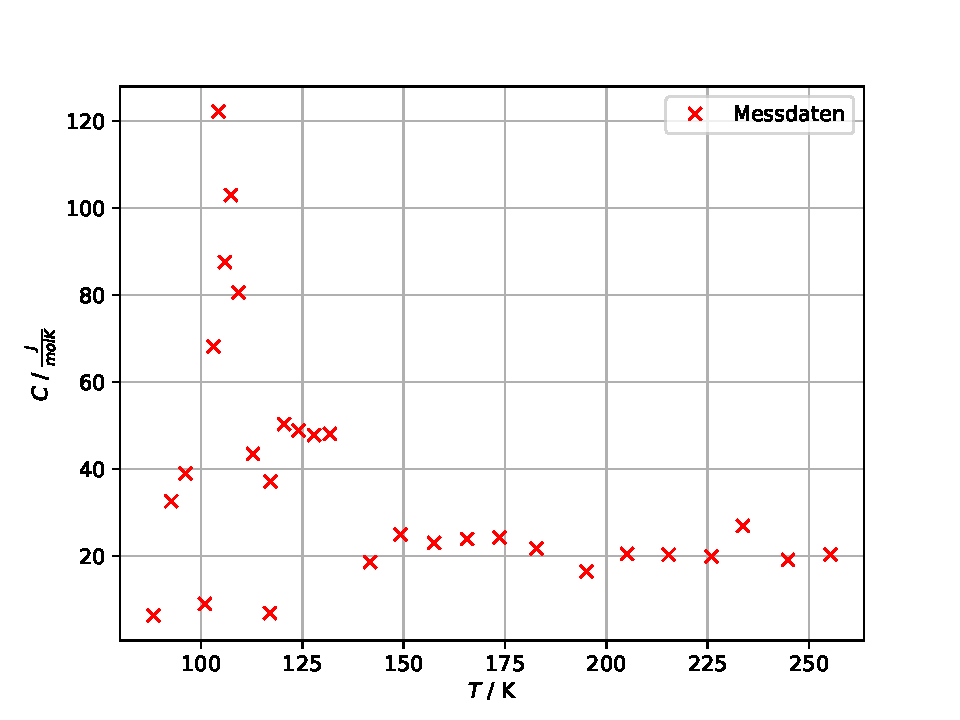
\includegraphics[width=0.7\linewidth]{../CvT2}
	\caption{Messdaten zu $C_V$ in Abhängigkeit der Temperatur $T$. Die blauen Linien markieren die Zeitpunkte an denen evakuiert und Stickstoff nachgefüllt wurde.}
	\label{fig:cvt2}
\end{figure}

\begin{figure}[h!]
	\centering
	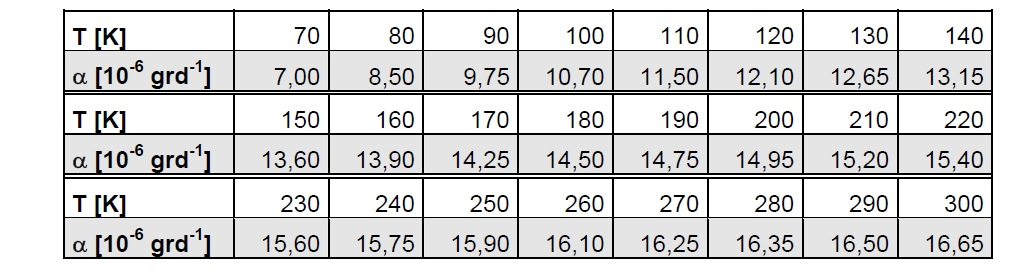
\includegraphics[width=0.7\linewidth]{../Tabelle2}
	\caption{Der lineare Ausdehnungskoeffizient von Kupfer, \cite[5]{anleitungV47}.}
	\label{fig:tabelle2}
\end{figure}

\subsection{Berechnung der Debye-Temperatur}

Im nächsten Auswertungsteil soll für die Wertepaare ($C_V$,T) eine geeignete Debye-Temperatur $\theta_\text{D}$ bestimmt werden. Es werden nur die Messwerte von $\SI{80}{\kelvin}$ bis $\SI{170}{\kelvin}$ berücksichtigt. Für die einzelnen errechneten $C_V$ Werte aus der Tabelle \ref{tab:cv} werden anhand der Abbildung \ref{fig:debyetemperatur} die zugehörigen $\frac{\theta_\text{D}}{T}$ Werte verglichen und bestimmt. Die so erhaltenden Werte werden mit der entsprechenden Temperatur multipliziert, um diese dann in Abbildung \ref{fig:debye} gegen die Temperatur aufzutragen. 

\begin{figure}[h!]
	\centering
	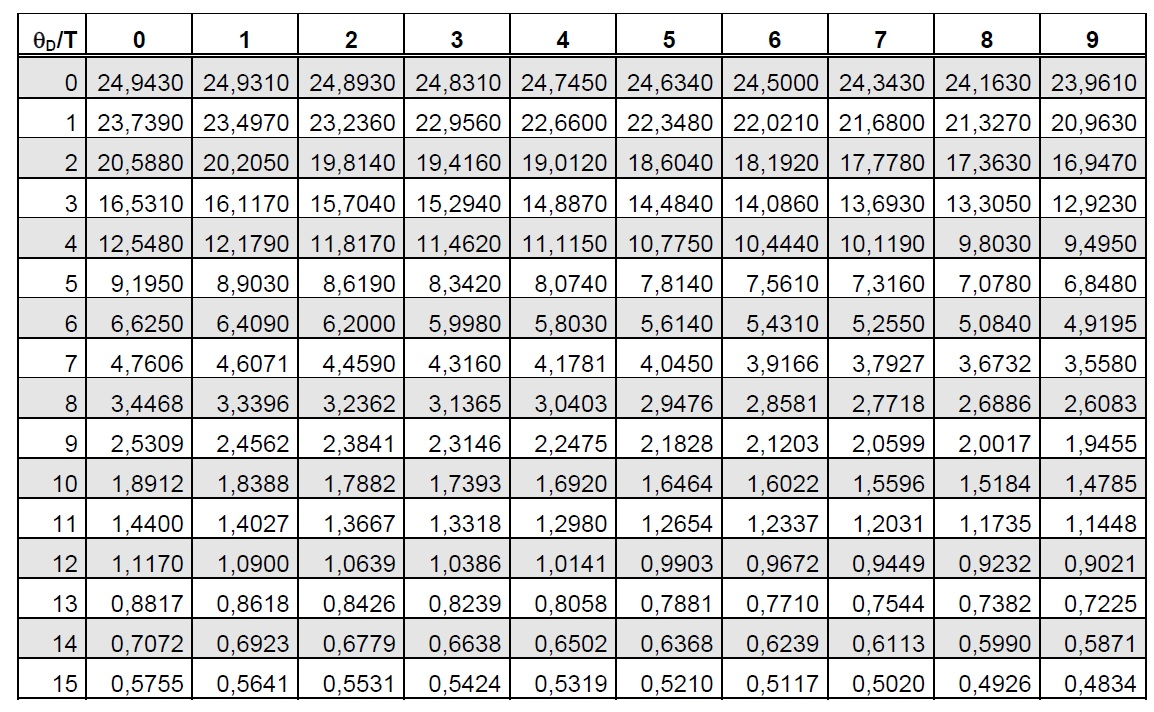
\includegraphics[width=0.9\linewidth]{../debyetemperatur}
	\caption{Zahlenwerte der Debye-Funktion, \cite[5]{anleitungV47}.}
	\label{fig:debyetemperatur}
\end{figure}

\begin{table}[htpb]
	\centering
	\caption{Debye-Temperatur.}
	\label{tab:thetad}
	\begin{tabular}{rrrr}
		\toprule
		$T/\si{\kelvin}$ & $C_V/ \si{\frac{\joule}{\kelvin \mol}}$ & $\frac{\theta_\text{D}}{T}$ & $\theta_\text{D}/\si{\kelvin}$\\
		\hline
		88,37	&	6,28	&	6,2 & 547,89	\\
		92,63	&	32,55	&	-	&	-\\
		96,18	&	38,88	&	-	&	-	\\
		117,01	&	6,85	&	5,8	& 678,65 \\
		100,93	&	8,97	&	5,0	& 504,05	\\
		103,06  &	68,20	&	-	&-	\\
		104,25	&	122,2	&	-	& -  \\
		105,92	&	87,60	&	-	&  - \\
		107,35	&	103,0	&	-	&-	\\
		109,26	&	80,60	&	-	&-	\\
		112,84	&	43,50	&	-	&-	\\
		117,15  &	37,20	&	-	& -  \\
		120,51	&	50,30	&	-	&  - \\
		124,11	&	48,88	&	-	&  - \\
		127,96	&	47,80	&	-	&  - \\
		131,81	&	48,10	&	-	&  - \\
		141,75	&	18,60	&	2,5	&  354,37 \\
		149,25	&	24,85	&	0,3	&  44,77 \\
		157,55	&	23,00	&	1,3	&  204,81 \\
		165,55	&   23,90	&	0,9	&  148,99 \\
		\bottomrule
	\end{tabular}
\end{table}

Aus dem Mittelwert und Fehler des Mittelwerts der in der Tabelle \ref{tab:thetad} angegebenen Werte für die Debye-Temperatur ergibt sich:
\begin{equation*}
\bar{\theta_\text{D}}= \SI{354,79 \pm 88,02}{\kelvin}
\end{equation*} 

\begin{figure}[h!]
	\centering
	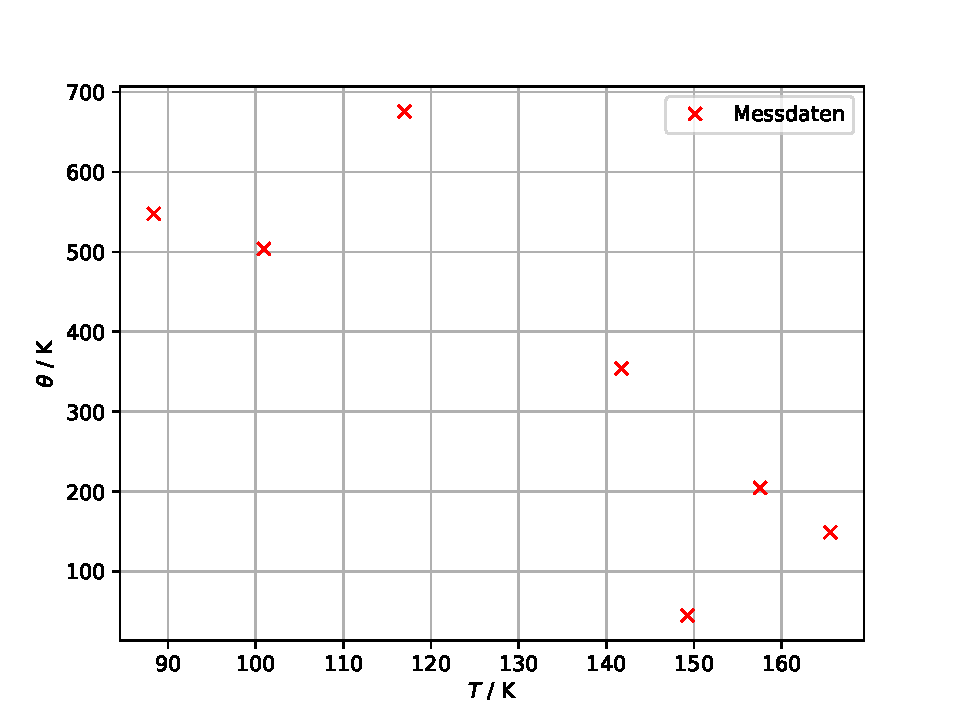
\includegraphics[width=0.7\linewidth]{../Debye}
	\caption{Messdaten zu $\theta_\text{D}$.}
	\label{fig:debye}
\end{figure}
\FloatBarrier

\subsection{Debye-Frequenz und theoretische Bestimmung der Debye-Temperatur}
Zuletzt werden die Debye-Frequenz $\omega_\text{D}$ und die Debye-Temperatur $\theta_\text{D}$ theoretisch bestimmt. Dafür wird die folgende Gleichung benötigt und umgeschrieben:
\begin{equation}
\omega_\text{D}^3=\frac{18\pi^2N_\text{A}}{V_0}\left(\frac{1}{v_\text{l}^3}+\frac{2}{v_\text{tr}^3}\right)^{-1}. \label{eqn:omegad}
\end{equation}
wobei $V_0$ das Molvolumen, $v_\text{l} = \SI{4,7E3}{\frac{\meter}{\second}}$ \cite[5]{anleitungV47} die Phasengeschwindigkeit einer longitudinalen Welle, $v_\text{tr} = \SI{2,26E3}{\frac{\meter}{\second}}$ \cite[5]{anleitungV47} die Phasengeschwindigkeit einer transversalen Welle und $N_\text{A} = \SI{6,022E23}{\frac{1}{\mol}}$ die Avogadro-Konstante \cite{AvogradoKonstante} sind. Es ergibt sich:
\begin{equation*}
\omega_\text{D} = \SI{4,349E13}{\frac{1}{\second}}
\end{equation*}
Damit lässt sich über der Gleichung:
\begin{equation}
\theta_\text{D} = \frac{\hbar \omega_\text{D}}{k_\text{B}}
\end{equation}
den theoretischen Wert für die Debye-Temperatur bestimmen. Die $k_\text{B}$-Konstante wird als Boltzmann-Konstante \cite{BoltzmannKonstante} bezeichnet. Es folgt:
\begin{equation*}
\theta_\text{theo-D} = \SI{332,18}{\kelvin}.
\end{equation*}
